%%%%%%%%%%%%%%%%%%%%%%%%%%%%%% -*- Mode: Latex -*- %%%%%%%%%%%%%%%%%%%%%%%%%%%%
%% arch.tex -- 
%% Author          : Joe Dane
%% Created On      : Tue Oct  5 15:34:23 1999
%% Last Modified By: Joe Dane
%% Last Modified On: Mon Nov  8 14:40:59 1999
%% RCS: $Id$
%%%%%%%%%%%%%%%%%%%%%%%%%%%%%%%%%%%%%%%%%%%%%%%%%%%%%%%%%%%%%%%%%%%%%%%%%%%%%%%
%%   Copyright (C) 1999 Joe Dane
%%%%%%%%%%%%%%%%%%%%%%%%%%%%%%%%%%%%%%%%%%%%%%%%%%%%%%%%%%%%%%%%%%%%%%%%%%%%%%%
%% 

\chapter{LOCC Architecture and Implementation}
\label{chap:arch}

LOCC provides both a tool for size counting and a set of ``shrink-wrapped'' 
size metrics.  This chapter will describe the design of the
various components which comprise LOCC.

LOCC is implemented as a Java application.  Presently, LOCC uses the 1.1
version of the Java language, and the 1.1.1 version of the Swing graphics
library.  A move to the Java2 platform is planned for the future. LOCC is
composed of a total of 76 classes, with a total of 555 methods and 8116
lines of code.  Figure \ref{fig:overview} shows a high-level overview of
the system.


The description of the architecture will proceed in three steps.
First, I will describe the interfaces which must be supported by size
counting code.  Second, I will discuss the classes comprising the user 
interface.  Finally, I will describe the code which implements the
default size counting for the Java language.
Comprehension of this chapter depends on a
familiarity with the basics of the Java language and with
object-oriented terminology in general.

\begin{figure}
\centering
%\vspace{4in}
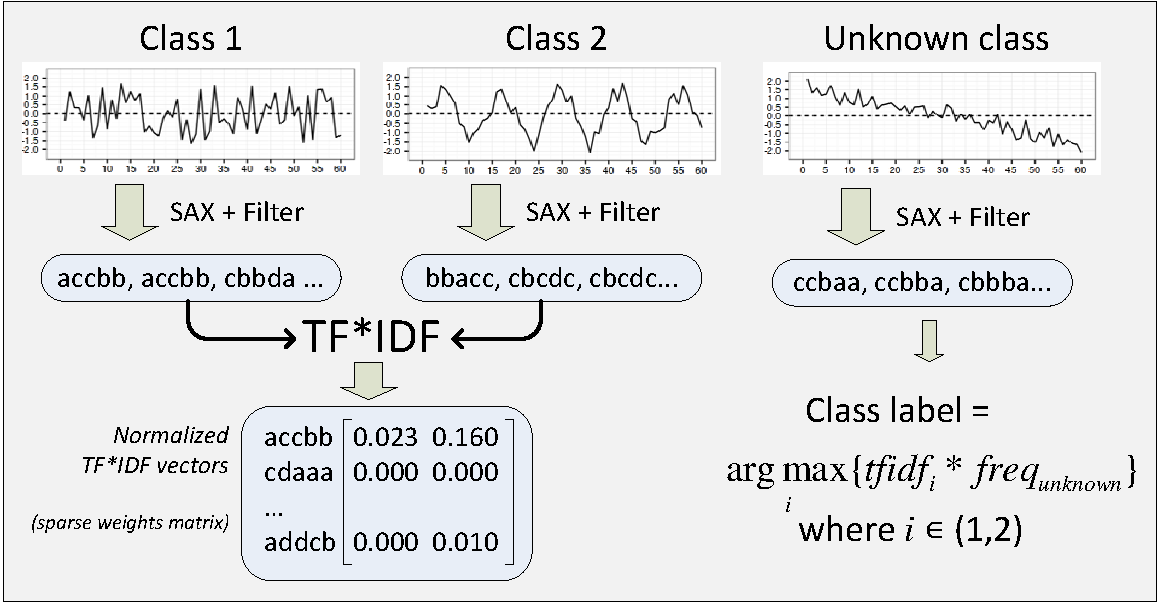
\includegraphics[angle=-90,width=\textwidth]{figs/overview.epsi}
\caption{Overview of the LOCC architecture}
\label{fig:overview}
\end{figure}

\section{Size counting interface}

The size counting interfaces are the means by which ``system'' code,
such as the command line parser and the GUI, invoke methods on code
which provide size counting services.  Since one of the primary goals of
LOCC is modularity, it is important that these interfaces be
general enough to support any size counting procedure imaginable.
A mechanism (which will be described in the user interface section
below) by which size counting code can be loaded at run time implies
that LOCC may not know at compile time which size counting modules
will be used at run time.  

\begin{figure}
\centering
%\vspace{3.5in}
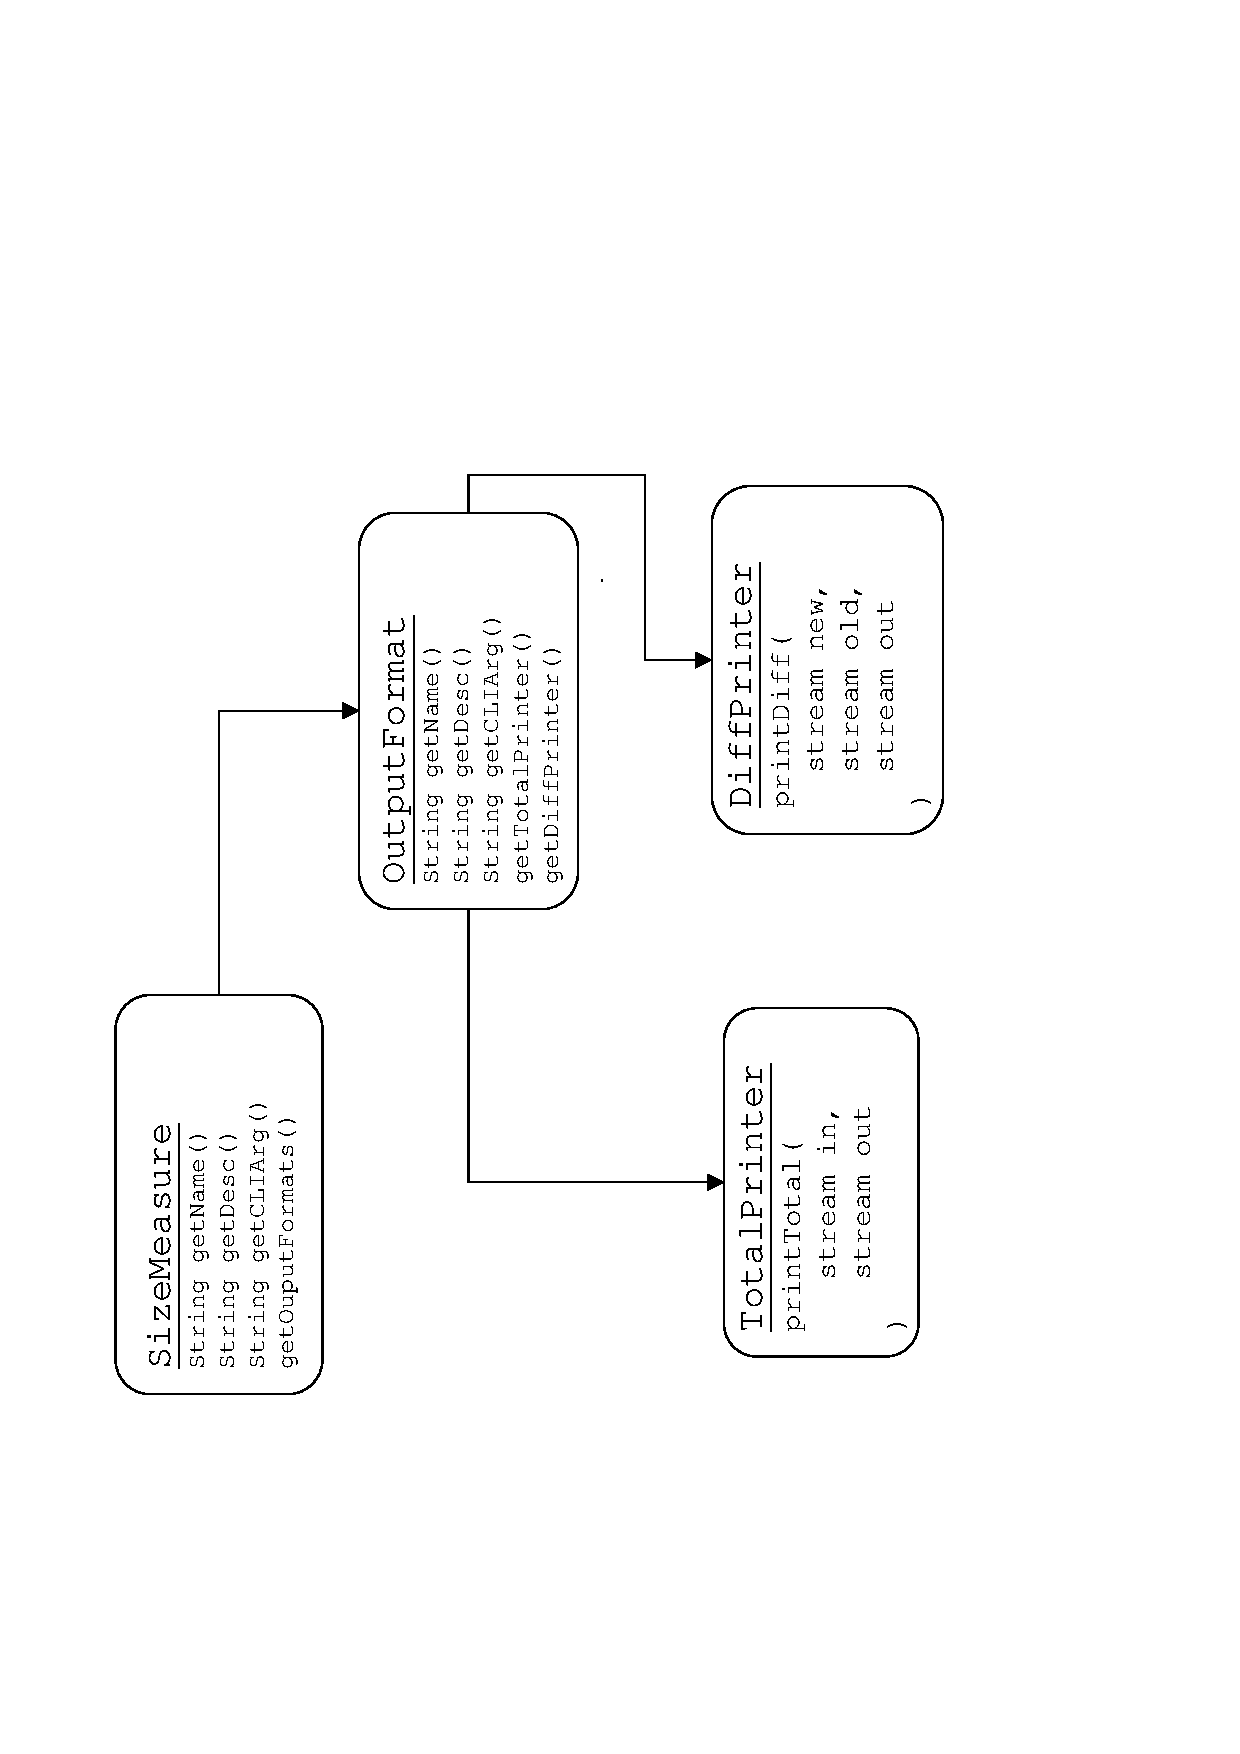
\includegraphics[angle=-90,width=\textwidth]{figs/size-measure.epsi}
\caption{LOCC size counting interfaces}
\label{fig:metric-interfaces}
\end{figure}

\subsection{The {\tt SizeMeasure} interface}

Figure \ref{fig:metric-interfaces} shows the relations between the four interfaces.  The
``top-level'' interface is \mbox{\tt SizeMeasure}, and this interface specifies
the following methods:

\begin{itemize}

\item \mbox{\tt String getName()}

This method should return a name for the size measure.  The name
should be short, but descriptive.  For example ``Java lines of code''.

\item \mbox{\tt String getCLIArg()}

This method should return a \mbox{\tt String} which will select the size measure
from the command line.  The \mbox{\tt String} should be all lowercase with no
spaces.  An example is \mbox{``{\tt javaline}''}.  No mechanism is in place for
detecting when two or more size measures declare the same argument
name.

\item \mbox{\tt String getDescription()}

This method should return a description of the size metric.  As the
result of this method is meant to be used in ``Help'' operations, the
message should be concise and clear.

\item \mbox{\tt OutputFormat[] getOutputFormats()}

Each \mbox{\tt SizeMeasure} is expected to provide its output in one or more
formats.  In practice, this usually means that output can be in a form 
suited for human consumption, or in a form meant to be used as the
input to some other tool\cite{Moore}.  This method returns an array of
objects implementing the \mbox{\tt OutputFormat} interface, described below.

\item Zero-argument constructor   

The \mbox{\tt SizeMeasure} must also include a zero-argument constructor.   The
Java language does not support the specification of constructors in
interface declarations, so this requirement is implicit.  It is
required because of the run-time code loading process described below.

\end{itemize}

\subsection{The {\tt OutputFormat} interface}

The \mbox{\tt OutputFormat} interface abstracts the behavior of code which
produces a single size measure with a single output format.  The
methods in the interface are:

\begin{itemize}

\item \mbox{\tt String getName()}

Returns a {\tt String} giving a short descriptive name for the output format, similar to the
method in \mbox{\tt SizeMeasure}.

\item \mbox{\tt String getCLIArg()}

Returns a \mbox{\tt String} used for selecting the output format at run time,
similar to the method in \mbox{\tt SizeMeasure}.

\item \mbox{\tt String getDescription()}

Returns a description of the \mbox{\tt OuputFormat}, similar to the method in
\mbox{\tt SizeMeasure}.

\item \mbox{\tt TotalPrinter getTotalPrinter()}
\item \mbox{\tt DiffPrinter getDiffPrinter()}

\end{itemize}

These methods return references to objects implementing the interfaces \mbox{\tt TotalPrinter}
and \mbox{\tt DiffPrinter}, respectively.  Methods on these objects are invoked
to count code.  There are several ``administrative'' methods in these
interfaces which will not be described here.  The two important
methods, implemented by \mbox{\tt TotalPrinter} and \mbox{\tt DiffPrinter} respectively, are

\begin{itemize}

\item
\singlespace
\begin{verbatim}
void printTotal(InputStream in, PrintWriter out) throws
  IOException, Parse Exception
\end{verbatim}
\doublespace 

\item 
\singlespace
\begin{verbatim}
void printDiff(InputStream new, InputStream old, 
               PrintWriter out) 
  throws IOException, ParseException
\end{verbatim}
\doublespace

\end{itemize}

\mbox{\tt printTotal} reads from its input and generates, by whatever means 
appropriate to the size measure and output format it supports, some
report on the size of what it has read.  In the process of generating
the size of the object read, it may encounter some exceptional
conditions.  If an error occurs in either read or writing, the method
can throw the standard Java exception \mbox{\tt java.io.IOException}.  If the
size measure is attempting to parse the input and is unable to
complete the parse, an exception \mbox{\tt csdl.locc.sys.ParseException} may be
thrown.  Since \mbox{\tt printTotal} and \mbox{\tt printDiff} are finally invoked by code in 
the user interface classes they can use these exceptions to
communicate information regarding the errors to the interface code,
where the information can be displayed to the user.  


Finally, note that there is no requirement that these interfaces be
implemented by distinct classes.  In some circumstances it may be
simpler to have a single class implement more than one, or even all,
of the interfaces.  See Chapter \ref{chap:add} for an example.


\section{User interface architecture}

A simplified class hierarchy for the LOCC user interface classes is shown
in Figure \ref{fig:user-graph}.

\begin{figure}
\centering
%\vspace{4in}
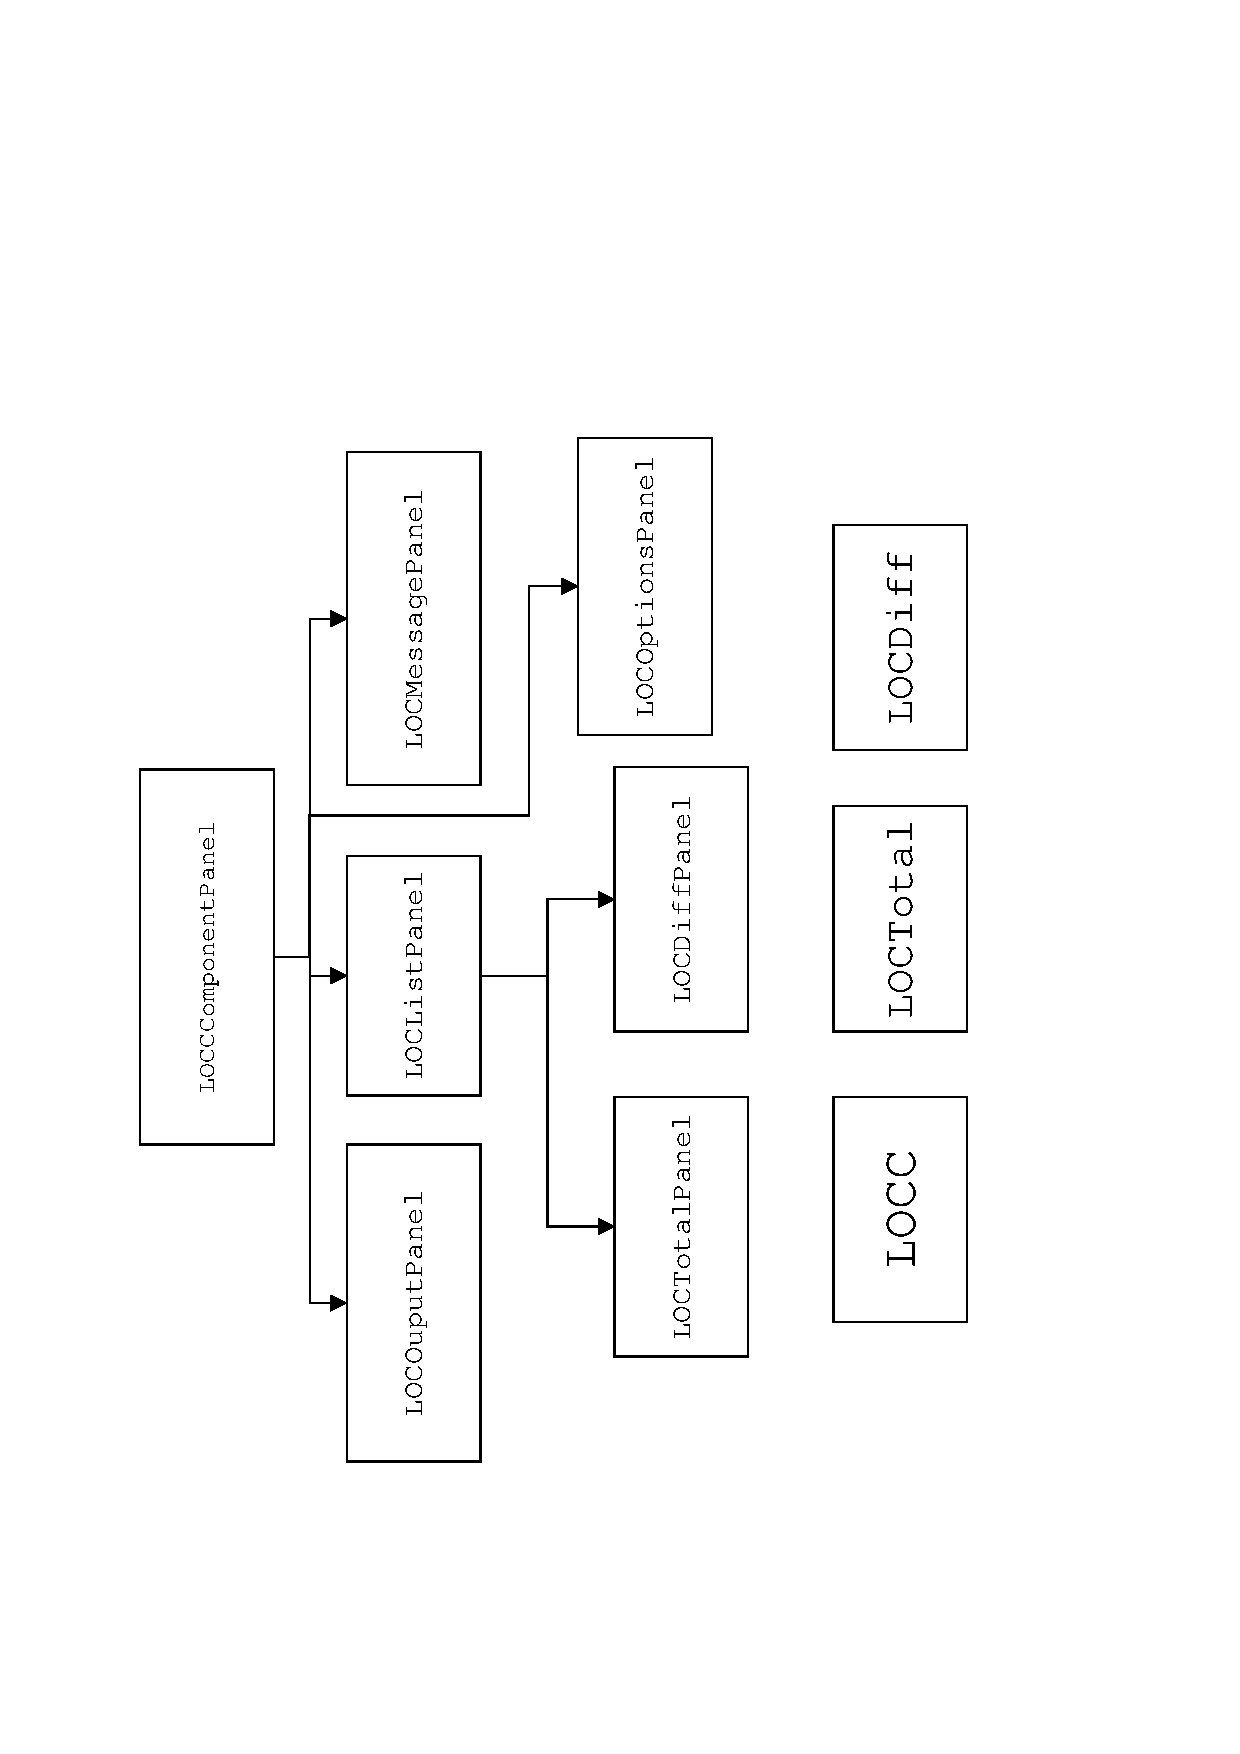
\includegraphics[angle=-90,width=\textwidth]{figs/locc-graph.epsi}
\caption{LOCC User interface classes}
\label{fig:user-graph}
\end{figure}

The class {\tt LOCC} is responsible for initializing the system, loading
size metrics, and displaying the main application window.  When the {\tt
  main} method of {\tt LOCC} is called, it will create a new top-level
window and add subclasses of the abstract class {\tt LOCComponentPanel} to
a tabbed panel.  

{\tt LOCComponentPanel} is an abstract base class which is extended by
classes wishing to display a panel within LOCC.  It arranges for event
handling to be set up, and imposes a single size on all its subclasses.

The classes {\tt LOCTotalPanel}, {\tt LOCDiffPanel}, {\tt LOCOuptutPanel},
{\tt LOCOptionsPanel} and {\tt LOCMessagePanel} are all subclasses of {\tt
  LOCComponentPanel}, and all define graphical screens in which input is
accepted  or output displayed.  {\tt LOCDiffPanel} and {\tt LOCTotalPanel}
are also subclasses of {\tt LOCListPanel}, which provides a list box which
can display the files to be processed.

The classes {\tt LOCTotal} and {\tt LOCDiff} contain methods to handle
command line invokation of total and difference counting, respecitvely.
They request that the {\tt LOCC} class load all size metrics but not
display a GUI.

\subsection{\mbox{\tt LOCCClassLoader}}

The \mbox{\tt LOCCClassLoader} class provides the glue which joins the interface
classes to the \mbox{\tt SizeMeasure} classes.  At system startup, LOCC looks for 
a properties file in certain defined locations.  The properties file
contains information about additional size metrics to be loaded at
run time.  The system creates an instance of \mbox{\tt LOCCClassLoader} to locate
and load these metrics.  No mucking about with a CLASSPATH variable is 
required, and the size metric classes can be installed anywhere on the 
system where the user invoking LOCC has read privilege.  For details on the 
format of the properties file, see Chapter \ref{chap:add}.



\section{Design of the Java LOC counter}

The most fully realized size metric currently shipping with LOCC is a
metric for counting Java source code.  This metric was designed to
suit the requirements of the Leap software development
toolkit\cite{Moore}, which was itself inspired by Watts Humphrey's
Personal Software Process\cite{Humphrey}.  Humphrey describes a regime for development
effort prediction which depends upon the developer having collected
data from past projects.  One of the measurements required is program
size.  The developer is required to break past projects into
``objects'', which in an object-oriented language such as Java
corresponds to classes, and to separate these objects into categories
depending on their size.  Size estimation for the current project
proceeds by categorizing the objects in the current design using the
developer's best guess as to which size category a particular object
will fall into when it is finally coded.  The size for the current,
projected object is then taken from the average size of the objects in 
the same category from the historical data set.

Leap takes a similar approach, but generalizes the ``object''
categorization into multiple, hierarchical size categories.  For
example, using the terminology of Java, methods can be considered the
atomic unit, with classes being composed of some number of methods,
and packages in turn composed of classes.  Leap is careful not to
impose this particular set of hierarchies, and leaves it up to the
developer to define the size hierarchy.  While the PSP uses lines of
code explicitly, Leap lets the developer use whatever unit he or she
wishes.  While Leap does not require it, the LOCC size
counter for Java, which will be referred to as {\sc javaline}, does use lines of code as its basic unit.  The
primary reason for this is consistency with the PSP, and also for the
general reasons described in Section \ref{why-loc}, chief among them
familiarity. 

{\sc javaline} is a realization of a Leap size hierarchy for Java code.  It
proceeds as described above, by collecting data for the three
hierarchical levels of methods, classes, and packages.  The Java
language complicates things slightly by allowing ``inner'' classes,
which can be declared within classes, methods, or even simple blocks.
These classes can themselves contain methods, which can contain
classes, and so on.  

{\sc javaline} take a practical approach to this complication, and others.  Only 
top-level classes are counted in the ``class'' level of the size
hierarchy.  The reason is that the entities counted at that level are 
meant to be characteristic of a certain entity in a design.
We are not so interested in the complexities of Java syntax as we are
in the process of proceeding from design to implemented product.  The
idea of a ``class'' is meant to abstract a certain design entity which 
maps most closely onto Java top-level classes.  

It could certainly be argued that some inner classes are themselves
complicated beasts, and as such should be conferred the same status as 
top-level classes.  While this may be true, {\sc javaline} takes the more
simplistic view that {\em in general} this is not the case, and that
an inner class should best be modeled as just another indistinguished
piece of code.

{\sc javaline} is composed of two parts: the total size
counter and the size difference counter.  They will be described
separately below.

\subsection{Java Total Size}

Total size counting for Java programs is fairly straightforward.  {\sc javaline}
includes a parser for version 1.1 of the Java programming language.
The parser was generated using the JavaCC parser
generator\cite{javacc-website}.

\subsubsection{Parsing Java source files}

A parse of a Java program proceeds as one would expect.  The 
only special actions taken are to keep track of which lines in the
input file contain Java code and which are empty or contain only
comments.  The JavaCC token manager makes this job fairly simple.  The 
result of the parse is an abstract syntax tree which has been
annotated with information to be used later.  The information kept
depends on the type of node in the tree.  Nodes representing Java
classes are annotated with the name of the class.  Method nodes are
annotated with the full signature of the method, to distinguish
overloaded methods.  If we are not interested in statement or
expression level constructs, these can be excluded from the generated
syntax tree. 

\subsubsection{Applying the Visitor}

{\sc javaline} utilizes the Visitor pattern\cite{Gamma} for traversing the
generated parse tree.  The reason for utilizing this pattern is
partially the conceptual cleanliness it imposes, and partially because 
JavaCC can be directed to automatically generate much of the code to
support the use of this pattern.

\begin{figure}
  \centering
  \input{JavaLineParserVisitor.java}
  \caption{The {\sc javaline} Visitor interface}
  \label{fig:visitor}
\end{figure}

In a Visitor pattern, an object designated the Visitor is applied to
the root node of a tree.  The Visitor can examine the state and
structure of the node, and can potentially recursively visit the
children of the node.  The pattern is expressed as 
a Java interface with one method, ``{\tt visit}'', which is overloaded for each
node type, as shown in Figure \ref{fig:visitor}. Code wishing to visit the nodes in 
a parse tree need simply to supply a behavior for the visitor at each
node type by implementing this interface.  The advantage of the Visitor
pattern is that the logic of the operation to be performed is kept in
separate Visitor classes, instead of in the syntax tree nodes.  Therefore,
the tree nodes can contain only the information specific to the node, and
different actions can be defined by providing different Visitors.  

The total size counter in LOCC supports two output formats: output in
a ``general'' human readable format, and output in a Leap data table
for input into Leap.  These formats are implemented as two Visitors.
The {\tt GeneralTotalVisitor}, for example, examines each node in a
parse tree, producing human readable output as it traverses the tree.


\subsection{Java Size Difference}

The difference counter in the {\sc javaline} metric is the result of
certain decisions described in this section.  The choices made were
motivated by the desire for the measured difference to correlate with the
amount of time spent in moving from one program version to another.

{\sc javaline} makes the following choice regarding the diff problem:

\begin{itemize}

\item Deleting code takes zero time.

\item Rearranging code takes zero time.

\item Adding new code takes non-zero time.

\end{itemize}

One complaint that could
be lodged against {\sc javaline} is that its is overly simplistic in its
treatment of deleted code.  Also, code added to a new version is given 
the same weight as the original code, when in fact much more thought
(and therefore time) might have gone into the new code, since it may
be constrained by the environment of the old code.  A developer has
fewer choices available when modifying existing code, which must
continue to support existing interfaces, than when developing an
entire product from the ground up.  It might be
reasonable to give added code a weight greater than unity.

It should be noted that while {\sc javaline}'s diff counter
does report differences in terms of syntactic units (new lines added
to each method, class, and package) this is not a requirement of
difference counting in general.  In measuring differences, we are usually
interested in how much a piece of code has changed, and not how much,
say, each method changed on average.  However, {\sc javaline} was designed
to be used within the Leap toolkit\cite{Johnson}, and Leap prefers its size 
measurements expressed in this manner.  As will be described below, this
causes some fairly significant problems.

\singlespace
\begin{figure}
  \centering 
  \begin{verbatim}
public class aClass {
    int i, j;
    public String methodOne() {
        return "methodOne";
    }
    public String methodTwo() {
        return "methodTwo";
    }
}
\end{verbatim}
  \caption{Old program version}
  \label{old-version}
\end{figure}

\begin{figure}
  \centering
  \begin{verbatim}
public class aClass {
    public String methodOne() {
        return "methodOne";
    }
    public String methodThree() {
        return "methodThree";
    }
    int i, j;
}
\end{verbatim}
  \caption{New program version}
  \label{new-version}
\end{figure}
\doublespace

Consider the program fragments in Figures \ref{old-version} and
\ref{new-version}.   
In going from the old version in Figure \ref{old-version} to the new
version in Figure \ref{new-version} three transformations have been applied.  First, a method
has been deleted.  Second, a new method has been added.  Finally, the
order of the declarations in the classes has been changed.  
When given these files as input, {\sc javaline} will
arrive at a total ``new'' size of 3 lines.


Java size difference counting begins in the same way as the total
count.  An abstract syntax tree is generated for both the old and new
versions of the program.  Then a Visitor is applied to the ``new''
tree and is passed the old tree as an argument.  

\subsubsection{What counts as a difference?}
\label{sect:whats-diff}
The difference Visitors work by utilizing the following
algorithm:

\begin{enumerate}
\item For the node currently being visited, look for a corresponding
  node in the old tree.  
\item If no match is found in the old tree, then the code is new.  Add 
  its lines to the total count and continue.
\item If a match is found, first recursively visit the children of the 
  node, looking for matches in the children of the old node.  Then
  produce a textual difference count of the text in the old and new
  nodes.
\end{enumerate}

The means of matching old and new nodes is worth looking at more
closely.  {\sc javaline} tries to do the best it can to make a sensible match.
For class nodes, {\sc javaline} will look for a class with the same name.  For
method node, {\sc javaline} will look for a method with the same signature, that 
is, a method of the same name with the same number and type of
arguments.  A problem arises  if the developer simply renames a
class or method and makes no other changes. {\sc javaline} will then be unable to
find a match in the old version and will consider the method or class
to be completely new.  This is probably the most serious fault in the
method {\sc javaline} uses, and will be discussed further in Chapter
\ref{chap:eval}. 

When two pieces of code are finally compared, a specialized hash table 
is used to determine the number of line differences.  The hash table
uses the text of the line of code as a key, and as a value the number of times the 
key has been added.  Multiple identical source lines are therefore
counted correctly.  Before being added to the hash table the line is
stripped of leading and trailing whitespace, in an attempt to minimize 
the effects of simply reformatting code.  Comments are also stripped
before the code enters the hash table, so the difference count is
insensitive to the addition or deletion of comments.

The question must naturally be asked, ``Since this matching business can be 
fooled by simply renaming a method, why bother with it at all?''  The
answer is that {\sc javaline} was meant to be used in conjunction with the
Leap toolkit, and the benefits of using an integrated toolkit such as Leap
were felt to outweigh the possible complications of this size metric.
It was also unknown when {\sc javaline} was designed how serious the
problem was.  If the problem occurred only rarely, then perhaps it would be
enough to let {\sc javaline} fail and manually correct the results.  As
will be discussed further in Chapter \ref{chap:eval}, it appears that the
problem is too serious to ignore.  Chapter \ref{chap:eval} will also discuss 
an alternative to {\sc javaline} which has been developed to alleviate the
problem.

\section{Other predefined size metrics}

LOCC currently ships with several predefined size metrics.  The {\sc
  javaline} metric has already been described.  There is a metric for
counting C++ code which operates in much the same way as {\sc javaline}.
Because the parser for the C++ size metric was written without regard to
current C++ standards, however, it should be considered less reliable at
this time.

LOCC additionaly contains metric to count statements and expressions in
Java source files.  These metrics are fully functional, in that they
contain methods to count both total size and size difference in terms of
statements or expressions.  However, when decisions had to be made in
designing the difference counters, the easy solution was always chosen.
Enhancing these metrics with more intelligent size difference measures is
one of the proposed future directions for LOCC.

LOCC also contains a size metric for counting plain ASCII text files.
There is nothing particularly interesting in the metric itself: it is
basically a reimplementation of the UNIX {\tt wc} and {\tt diff}
utilities.  The ASCII text metric is interesting because is suggests a
wider application domain for LOCC.  Instead of being exclusively a tool for 
measuring the size of software products, LOCC can be utilized to measure
the size of any work product.  For example, one may wish to keep track of
the size of a paper or proposal being composed.  The same productivity
measures and time estimation procedures used in software development can be 
used in these non-software development environments.  
